% AutoUI Work-in-Progress draft.
% Target venue: AutomotiveUI WIP track. Keep main text within the WIP page limit.
\documentclass[sigconf,review,anonymous]{acmart}
\settopmatter{printacmref=true}
\renewcommand\footnotetextcopyrightpermission[1]{}
\microtypesetup{expansion=false}
\hypersetup{%
  pdftitle={Auditable Driver-State Annotation from Naturalistic In-Cabin Video},
  pdfauthor={Anonymous Author(s)},
  pdfkeywords={Naturalistic driving, driver monitoring, glance annotation, human-in-the-loop, area of interest, hand-on-wheel}}
\acmConference[AutomotiveUI WIP]{AutomotiveUI Work-in-Progress Track}{2026}{}
\acmBooktitle{AutomotiveUI Work-in-Progress Track, 2026}
\acmYear{2026}
\copyrightyear{2026}
\setcopyright{none}
\acmDOI{}
\acmISBN{}
\newcommand{\autouitablefont}{\footnotesize}

\begin{document}

\title{Auditable Driver-State Annotation from Naturalistic In-Cabin Video}

\author{Anonymous Author(s)}
\affiliation{%
  \institution{Anonymous Institution}
  \city{Anonymous}
  \country{Anonymous}}
\email{anonymous@example.com}

\begin{abstract}
Naturalistic driving studies often rely on in-cabin video to study driver
attention and supervision, yet many datasets lack synchronized eye
tracking or frame-level driver-state labels. This creates a measurement
gap for downstream behavioral analysis: researchers need scalable
features that describe where drivers look and whether their hands remain
on the steering wheel, but fully manual coding does not scale to long
recordings with many participants. This work-in-progress paper presents
an auditable human-in-the-loop workflow that converts ordinary in-cabin
video into area-of-interest (AOI) glance categories and hand-on-wheel
state variables. The workflow combines reviewed driver ROI
specification, consensus AOI annotation, participant calibration,
frame-level inference, temporal stabilization, hand/wheel detection,
state distillation, and window-level metric extraction. We report
preliminary evidence from 15 participants, including 301 processed
gaze/wheel segments, about 3.91 million frame-level outputs, 7,306
coverage-qualified behavior windows, a 14-participant AOI
leave-one-participant-out experiment, a few-shot adaptation curve, a
temporal stabilization ablation, hand-on-wheel review subsets, a
teacher-student hand-state distillation check, and ONNX deployment
checks. The contribution is not a new gaze backbone or an eye-tracking
replacement. Instead, the paper defines a reusable annotation and
validation workflow for downstream studies that require transparent,
reviewable driver-state features from naturalistic video.
\end{abstract}

\begin{CCSXML}
<ccs2012>
   <concept>
      <concept_id>10003120.10003121.10011748</concept_id>
      <concept_desc>Human-centered computing~Empirical studies in HCI</concept_desc>
      <concept_significance>500</concept_significance>
   </concept>
   <concept>
      <concept_id>10010147.10010371.10010396</concept_id>
      <concept_desc>Computing methodologies~Computer vision tasks</concept_desc>
      <concept_significance>300</concept_significance>
   </concept>
</ccs2012>
\end{CCSXML}

\ccsdesc[500]{Human-centered computing~Empirical studies in HCI}
\ccsdesc[300]{Computing methodologies~Computer vision tasks}

\keywords{Naturalistic driving, driver monitoring, glance annotation, human-in-the-loop, area of interest, hand-on-wheel}

\maketitle

\section{Introduction}

Naturalistic driving studies preserve real traffic, cabin layouts,
lighting, and driver behavior, but many in-cabin video datasets are
recorded with ordinary cameras rather than synchronized eye trackers.
They therefore lack fixations, point-of-regard estimates, and
area-of-interest (AOI) glance labels. Before such datasets can support
questions about monitoring, distraction, takeover readiness, or
automation engagement, researchers must first turn video into behavioral
variables.

Manual coding is interpretable but difficult to scale because it requires
coder training, consensus review, and reliability audit. Fully automated
vision is attractive, but a black-box classifier is not sufficient for
naturalistic driving data: a prediction can be invalid when the driver
crop is wrong, a passenger appears in the selected region, a face detector
fails, or short flicker is interpreted as a behavioral event.

Prior work motivates coarse regions and behavioral states rather than
exact gaze or hand geometry. Video-based driver visual behavior standards
define glance measures as observable AOI episodes and durations
\cite{saeJ2396,iso15007}. Gaze-region work shows that head pose,
eye-region appearance, and scene geometry can support roadway or
in-vehicle glance classification without eye tracking
\cite{fridman2016drivergaze,fridman2016robustgaze}. For steering
engagement, recent work has studied driver hand detection, synthetic
hands-on-wheel data, and in-vehicle hands on/off prediction
\cite{borghi2018handswheel,yudkin2022handsup,pyeon2023handsonoff}.
Our contribution is complementary: we do not claim a new detector or an
external benchmark result, but define an auditable workflow that turns
ordinary naturalistic in-cabin video into documented AOI and hand-state
features.

We therefore treat driver-state extraction as a measurement workflow
rather than a single model score. YOLOv8-cls provides a compact
train-export-deploy path \cite{jocher2023ultralytics}; SCRFD supports
driver ROI review \cite{guo2021scrfd}; and GroundingDINO localizes
text-prompted hands and steering wheels \cite{liu2023groundingdino}.
Humans still define the study geometry and semantics: they confirm driver
regions, label AOIs, review outputs, and inspect uncertain hand states.

The resulting measures are AOI-level driver-state features, not
continuous gaze estimates or eye-tracking substitutes
\cite{fridman2016drivergaze,saeJ2396,iso15007}. This WIP defines the
workflow, reports preliminary checkpoint evidence from 15 participants,
evaluates model/deployment choices, and adds a state-distillation
checkpoint for the slow hand/wheel branch before any large-scale student
replacement is claimed.

\section{Method}

Figure~\ref{fig:workflow} summarizes the workflow. The input is a set of
target videos and analysis segments defined by a study spreadsheet. The
workflow resolves local videos, assigns or reviews driver regions,
constructs annotation packs, collects human AOI labels, trains
participant-specific AOI classifiers, exports deployment models, runs
segment-level inference, stabilizes frame-level predictions, estimates
hand-on-wheel states, optionally distills GroundingDINO teacher outputs
into a lightweight state student, and aggregates the resulting streams
into behavioral windows.

\begin{figure}[t]
    \centering
    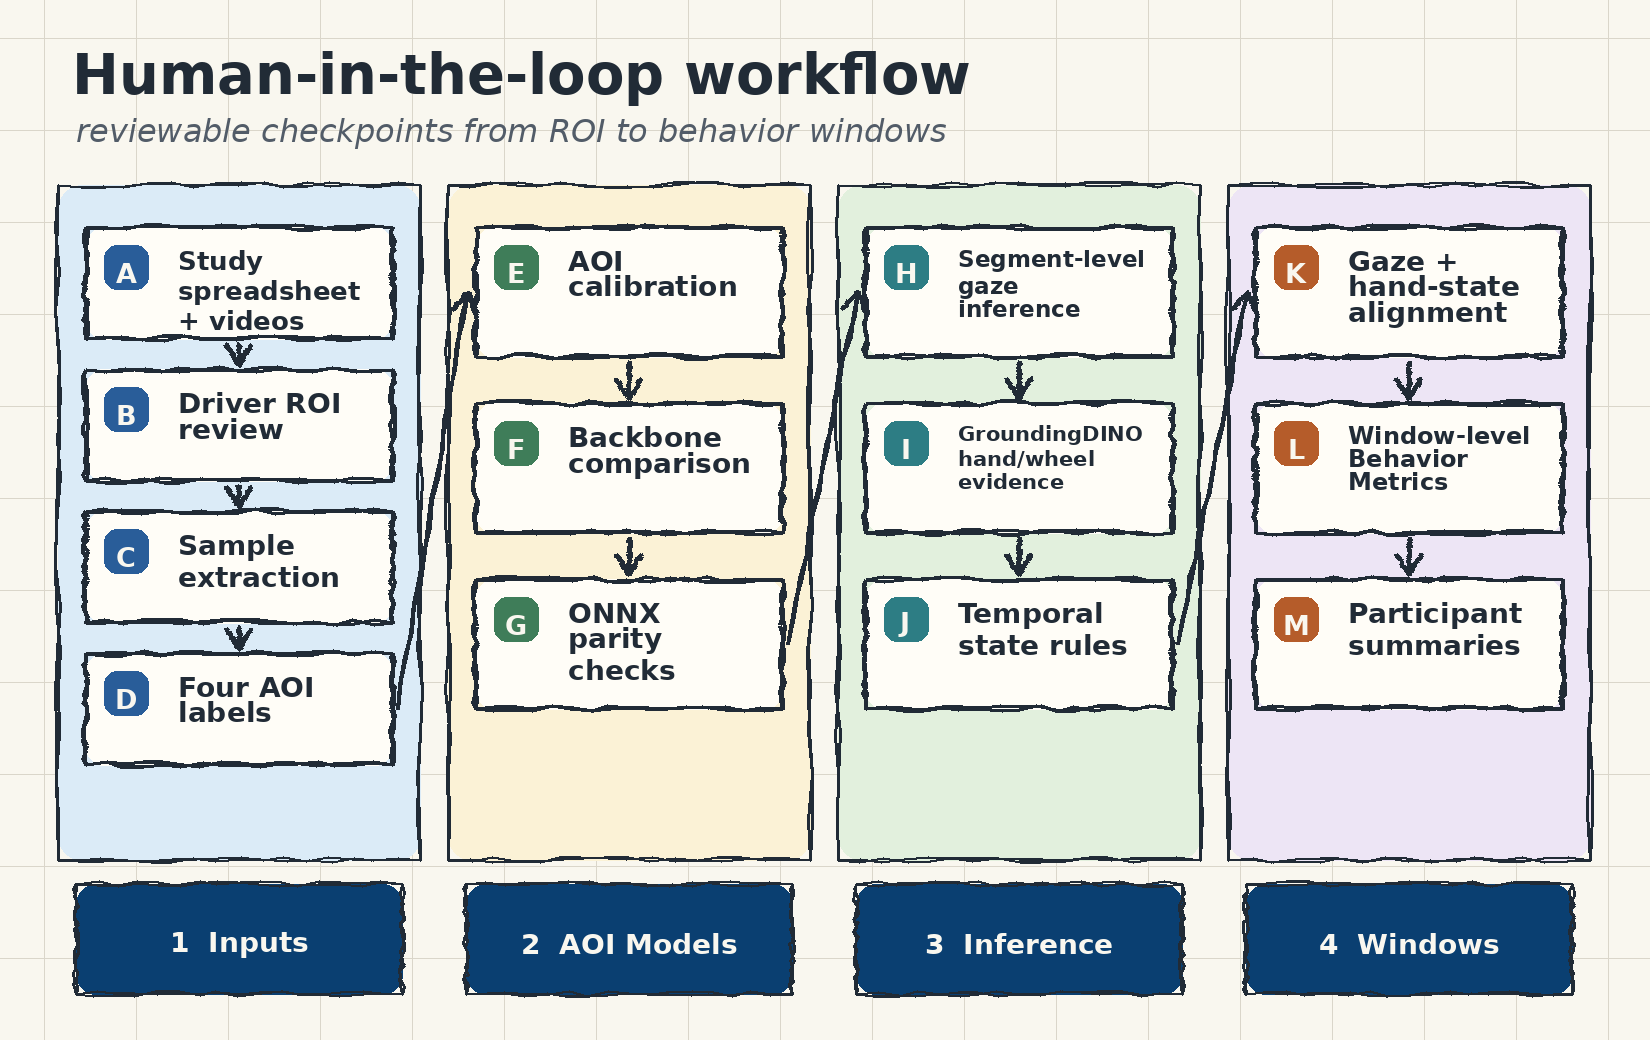
\includegraphics[width=\linewidth]{figures/label_workflow.png}
    \Description{A workflow diagram showing spreadsheet-defined target videos,
    human ROI specification, annotation packs, AOI model training, ONNX
    export, segment inference, temporal stabilization, and window-level
    behavior aggregation.}
    \caption{Human-in-the-loop workflow for deriving AOI-level glance and
    hand-on-wheel variables from naturalistic in-cabin video. The method keeps
    ROI provenance, frame semantics, temporal stability, hand-state review, and
    behavior aggregation as separate reviewable stages.}
    \label{fig:workflow}
\end{figure}

\subsection{Measurement Targets}

The gaze branch assigns each interpretable frame to one of three valid
AOI classes. \textit{Forward} denotes attention toward the forward
roadway. \textit{In-Car} denotes attention toward in-vehicle targets such
as the instrument cluster, center display, mirrors, or controls.
\textit{Non-Forward} denotes attention away from both the forward roadway
and in-vehicle targets. A fourth label, \textit{Other}, is used for
invalid or non-interpretable frames. Primary behavior metrics use the
three valid AOI classes, while \textit{Other} is retained for cleaning,
model training, and secondary error analysis.

The hand branch estimates steering-wheel engagement as \textit{ON},
\textit{OFF}, or \textit{UNCERTAIN}. These states are derived from hand
and steering-wheel detections, spatial contact evidence, and temporal
state rules. For window-level analysis, hand-state samples are aligned
with the gaze stream so that researchers can compute both overall and
AOI-conditioned hands-on/off ratios.

\subsection{Human ROI and AOI Annotation}

ROI selection is part of the measurement method, not an invisible
preprocessing step. Reviewers record simple driver ROIs directly; in
dual-panel or multi-view layouts, face evidence ranks candidate panels
but the selected panel remains visually confirmed. Uncertain assignments
export grid-overlay references and fill-in manifests for manual
correction.

After ROI specification, representative frames are sampled across each
target video and coded as \textit{Forward}, \textit{In-Car},
\textit{Non-Forward}, or \textit{Other}. The \textit{Other} class
captures systematic invalid samples from occlusion, lighting, camera
layout, or non-driver faces, preventing these frames from contaminating
valid AOI metrics.

The annotation process preserves consensus decisions while keeping
reliability audit as an explicit WIP activity. Coders are trained on a
shared manual and exemplar frames, production labels are reviewed before
consensus, and disagreements are resolved through joint discussion.
Chance-corrected reliability indices such as Cohen's \(\kappa\)
\cite{cohen1960coefficient} are useful when a completed double-coded
audit set is available; Fleiss' \(\kappa\) is appropriate only when more
than two coders independently label the same items \cite{fleiss1971}.
Because the present WIP is still in the feature-construction stage, we
treat aggregate agreement as descriptive process evidence and leave the
formal chance-corrected reliability audit for the next validation pass.

\subsection{AOI Classification and Temporal Stabilization}

The operational AOI branch uses a YOLOv8-cls classifier because it
provides a compact training and deployment path. Participant-specific
calibration starts from a small set of labeled samples and produces a
participant-adapted classifier for segment-level inference. At inference
time, SCRFD detects faces within the reviewed driver ROI; a
layout-specific target-face rule rejects implausible identity jumps and
selects the driver face; the selected crop is then classified into the
four AOI labels.

Deployment convenience does not by itself establish measurement validity.
For that reason, the repository also includes a model-comparison workflow
that trains YOLOv8-cls, ResNet, EfficientNet, ConvNeXt, and ViT backbones
under a common participant holdout protocol. The comparison is not meant
to find a universal best backbone; it tests whether the deployment choice
has an irreplaceable accuracy advantage under generalization and
calibration constraints.

Frame-level outputs are not used directly as behavioral events. Presence
hysteresis prevents brief missed detections from producing invalid
states, and class debounce requires a candidate AOI label to persist
before replacing the current stable label. This keeps frame semantics and
temporal event structure analytically distinct.

\subsection{Hand-on-Wheel State Estimation}

The hand branch uses the steering-wheel camera view. GroundingDINO
detects hands and steering wheels with text prompts. Contact
evidence is computed from overlap between detected hand boxes and
steering-wheel boxes. The frame-level state machine maps reliable contact
evidence to \textit{ON} or \textit{OFF}; unreliable frames retain the
previous state for a short grace period before entering
\textit{UNCERTAIN}. A temporal majority rule then produces the stable
state sequence used for review and metric extraction.

GroundingDINO is useful for text-prompted bootstrapping but too slow for
repeated large-scale processing, so it is treated as a teacher detector.
Sampled teacher detections can supervise either a two-class hand/wheel
detector student or, as used here, a state-level ROI-crop classifier
supervised by stable \textit{ON}/\textit{OFF}/\textit{UNCERTAIN} outputs.
This branch is reviewed at the final-state level, after detector
confidence, contact rules, and temporal stabilization act together.

\subsection{Window-Level Metrics}

The stabilized gaze and hand-state streams are aggregated into fixed
analysis windows. The window is not a new labeling task; it is a
deterministic, timestamp-weighted aggregation of the stabilized AOI and
hand-state streams. This design reduces the influence of short-term
prediction flicker, matches the downstream 20 s analysis unit, and keeps
each derived value traceable to frame-level states, valid denominators,
coverage gates, and episode-duration rules. Let \(g_i\) be the stabilized
AOI label at time \(t_i\) and let \(\mathcal{L}=\{\textit{Forward},
\textit{In-Car}, \textit{Non-Forward}\}\) be the valid AOI set. Samples
labeled \textit{Other} are excluded from valid-AOI denominators. AOI time
percentages use timestamp-based frame-duration weights rather than raw
frame counts.

Glance counts are computed as entries into AOI episodes. Consecutive
frames with the same valid AOI label are treated as one episode. Long
off-path glances are defined as consecutive frames in either
\textit{In-Car} or \textit{Non-Forward}, with event counts reported at
1.6 s and 2.0 s thresholds. Hand-on-wheel ratios are computed overall and
conditioned on AOI label after excluding \textit{UNCERTAIN} and unmatched
wheel-state samples. Windows failing the gaze-coverage threshold are kept
for QC but excluded from participant-level summaries.

\section{Experiments}
\label{sec:preliminary_validation}

The evaluation focuses on whether the workflow produces reviewable
measurement artifacts, not whether it solves driver monitoring in a
single end-to-end score. Unless otherwise stated, evidence reflects
artifacts finalized by May 24--25, 2026 for the 15-participant analysis
set.

\begin{figure}[t]
    \centering
    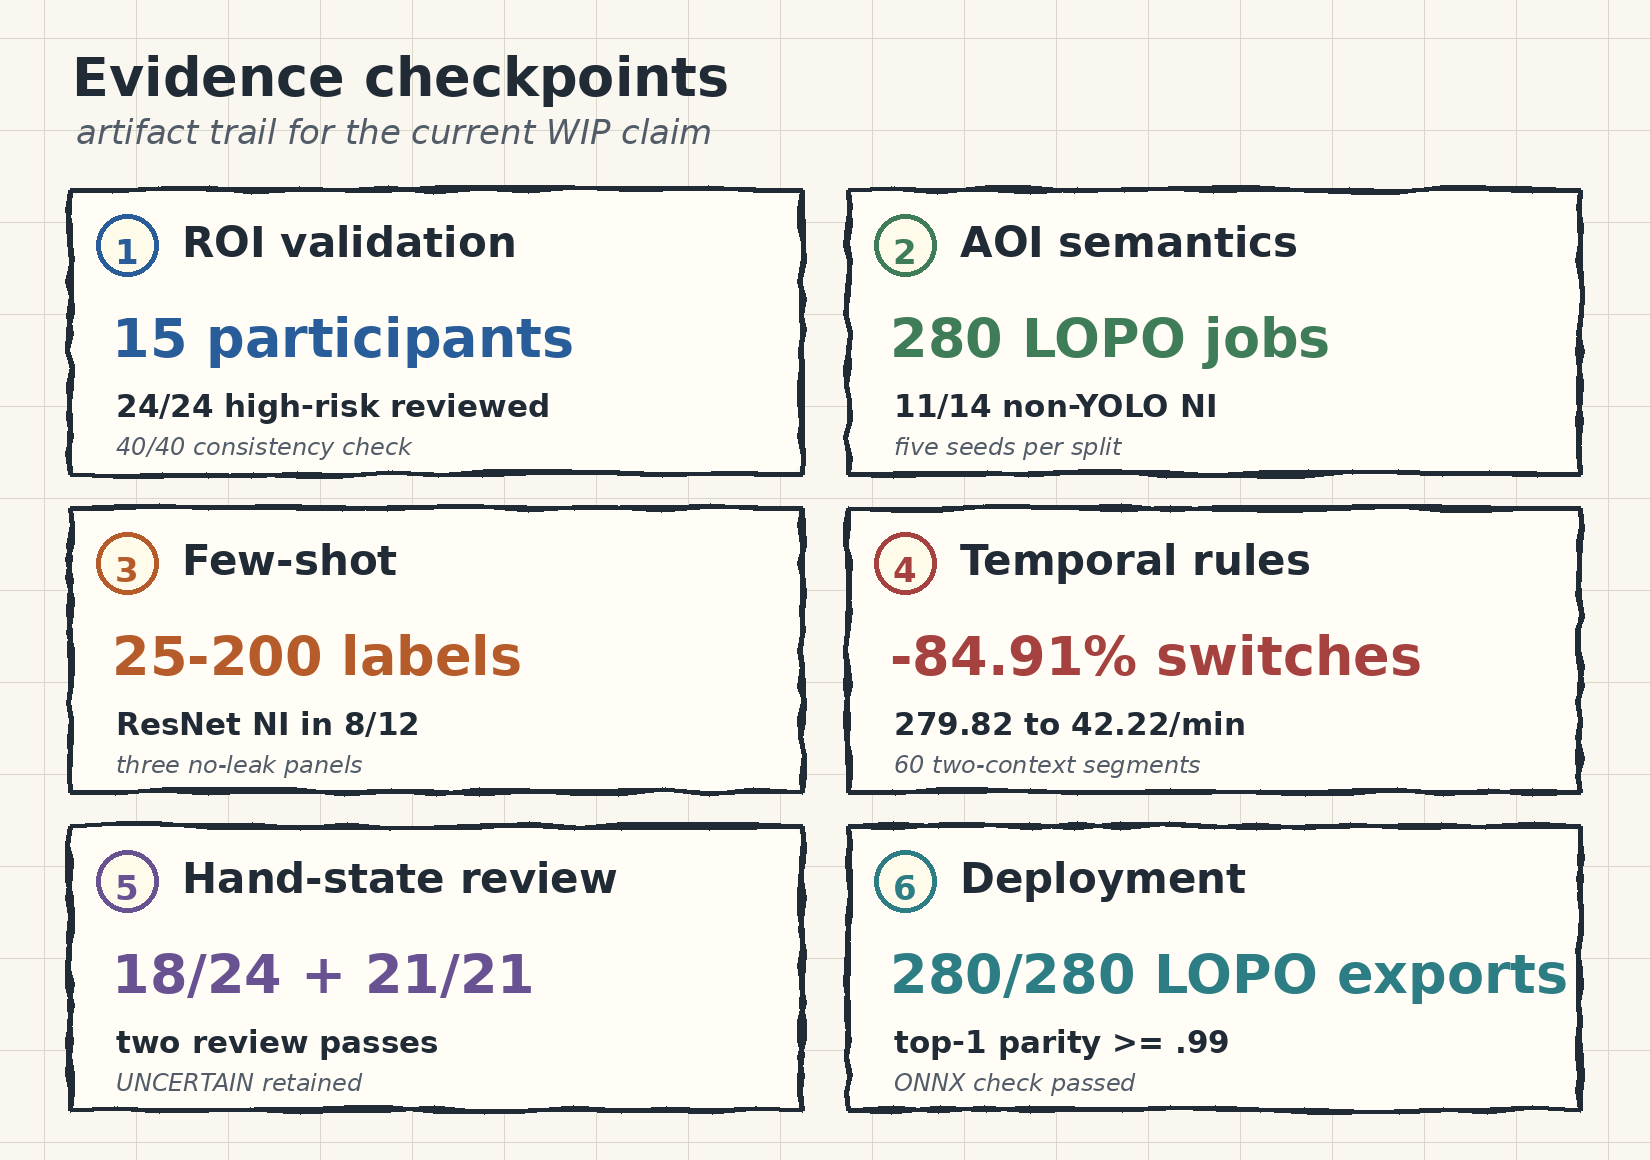
\includegraphics[width=\linewidth]{figures/evidence_checkpoints.png}
    \Description{A hand-drawn style diagram with six checkpoint boxes:
    ROI validation, AOI semantics, few-shot adaptation, temporal stability,
    hand-state review, and deployment. Each box contains a headline result
    from the evaluation artifacts.}
    \caption{Evidence checkpoints used to evaluate the annotation workflow.
    Each checkpoint corresponds to a distinct source of possible measurement
    error.}
    \label{fig:evidence_checkpoints}
\end{figure}

\subsection{ROI and Processing Coverage}

The ROI branch covers 15 participants with human-specified or
human-confirmed ROI assignment files and production gaze/wheel ROI
manifests. The completed audit covered provenance, resolution, visual
validity, uncertain dual-ROI rows, low-margin detector-assisted rows, and
layout-specific gaze/wheel checks. All 24 high-risk rows were resolved,
and a manual/current ROI consistency check matched 40/40 rows with zero
coordinate changes.

The rebuilt inference plans, gaze maps, wheel maps, and 20 s behavior
windows cover all 15 analysis participants. Table~\ref{tab:coverage_refresh}
summarizes the resulting processing coverage. All 301 planned gaze/wheel
segments had frame-level CSV outputs, and all 7,327 generated windows
resolved to gaze and wheel files. The final participant-level summaries
used 7,306 windows passing the 0.98 gaze-coverage threshold; 21 windows
were retained for QC only.

\begin{table}[t]
\centering
\caption{Processing coverage across the 15-participant analysis set.}
\label{tab:coverage_refresh}
\autouitablefont
\begin{tabular}{lr}
\toprule
Coverage item & Value \\
\midrule
Participants in analysis & 15 \\
Matched target videos & 176 \\
Gaze segments with CSV outputs & 301 \\
Wheel segments with CSV outputs & 301 \\
Frame-level gaze rows & 3,914,416 \\
Frame-level wheel-state rows & 3,914,412 \\
Generated 20 s windows & 7,327 \\
Coverage-qualified windows & 7,306 \\
QC-excluded windows & 21 \\
\bottomrule
\end{tabular}
\end{table}

\subsection{AOI Generalization and Adaptation}

To evaluate cross-participant generalization, we ran a 14-participant
leave-one-participant-out (LOPO) AOI experiment with five seeds and four
backbones, for 280 training runs. The primary metric is three-class
macro-F1 over \textit{Forward}, \textit{In-Car}, and
\textit{Non-Forward}; \textit{Other} remains a secondary data-quality
label because current test sets have limited invalid-sample support.

All training and prediction jobs completed. Table~\ref{tab:lopo_means}
reports mean held-out performance across the 70 runs per model. ResNet50
achieved the highest mean metrics; YOLOv8s-cls remains useful for
deployment but was not uniquely accurate.

\begin{table}[t]
\centering
\caption{Mean held-out performance in the five-seed 14-participant LOPO
AOI experiment. Each model has 70 held-out runs.}
\label{tab:lopo_means}
\autouitablefont
\begin{tabular}{lrrr}
\toprule
Model & Macro-F1 & Bal. acc. & Event acc. \\
\midrule
ResNet50 & 0.596 & 0.625 & 0.627 \\
EfficientNet-B0 & 0.575 & 0.601 & 0.616 \\
YOLOv8s-cls & 0.574 & 0.606 & 0.618 \\
DeiT-Tiny & 0.300 & 0.350 & 0.399 \\
\bottomrule
\end{tabular}
\end{table}

At the split level, the best non-YOLO mean exceeded YOLOv8s-cls on 11/14
participants. A 3 percentage-point bootstrap non-inferiority test found
at least one non-YOLO candidate satisfying the margin on 11/14 splits,
supporting family-best non-inferiority rather than exact equivalence.

The few-shot experiment tests how much participant-specific labeling is
needed when the goal is adaptation rather than zero-label
generalization. We ran a no-leak adaptation curve over three
participant-specific adaptation panels at 25, 50, 100, and 200 label
budgets, five seeds per budget, and frozen participant-specific test
sets. Figure~\ref{fig:fewshot_curve} shows rapid ResNet50 gains from 25
to 100 labels and YOLOv8s-cls leading at 200 labels. ResNet50 was
non-inferior to YOLOv8s-cls in 8/12 participant-budget cells, suggesting
that label budget should be controlled and reported.

\begin{figure}[t]
    \centering
    
\includegraphics[width=\linewidth]{figures/fewshot_curve.png}
    \Description{A hand-drawn style line chart showing ResNet50 and
    YOLOv8s-cls macro-F1 over 25, 50, 100, and 200 participant-specific
    labels. ResNet50 rises quickly through 100 labels and YOLOv8s-cls is
    highest at 200 labels.}
    \caption{Few-shot no-leak adaptation curve over three
    participant-specific adaptation panels (five seeds per
    participant-budget cell).}
    \label{fig:fewshot_curve}
\end{figure}

\subsection{Temporal Stability}

We compared raw per-frame AOI predictions with stabilized
\textit{Gaze\_Class} on a two-context subset covering 60 segments,
643,603 frames, and 436.95 min. Stabilization reduced label switches from 279.82
to 42.22 per minute, an 84.91\% reduction. Raw and stable labels
differed on 106,418 frames, or 16.54\% of the subset. Stabilization also
changed behavior-level event structure: 1.6 s off-path episodes rose
from 923 to 1,289, and 2.0 s episodes rose from 696 to 1,032, showing
that temporal rules change event structure rather than cosmetic
smoothness alone.

\subsection{Hand-State Review and Distillation}

The wheel branch produced 301 segment-level outputs and 3,914,412
state-classified rows. Several driver/camera contexts had
majority-\textit{UNCERTAIN} support, indicating that hand-state
estimation is sensitive to camera layout, occlusion, and steering-wheel
evidence. AOI/glance metrics can be used independently; hand-conditioned
metrics should report the valid \textit{ON}/\textit{OFF} denominator, and
majority-\textit{UNCERTAIN} contexts should be treated as low-support hand
evidence.

The first agreement summary contained 24 reviewed rows with matched
pipeline and human labels. Agreement was 18/24 (75.0\%), with four
false-ON and two false-OFF cases. During review, we found that one
evidence batch initially reused single-panel gaze ROIs as wheel ROIs. We
therefore regenerated layout-specific cockpit evidence for the affected
participants. The corrected second pass covered 21 final states; the
reviewer matched all 21 pipeline states, including 12 binary ON/OFF cases
and nine \textit{UNCERTAIN} cases (Table~\ref{tab:wheel_second_pass}).
We interpret this second pass as a post-correction workflow sanity check
showing that the regenerated evidence is internally consistent with
reviewed final states, not as an independent human-gold-standard
validation of hand-state measurement.

\begin{table}[t]
\centering
\caption{Hand-on-wheel final-state validation outcomes.}
\label{tab:wheel_second_pass}
\autouitablefont
\begin{tabular}{lrrr}
\toprule
Scope & Reviewed & Agreement & False ON/OFF \\
\midrule
Initial manifest & 24 & 18/24 & 4/2 \\
Corrected second pass & 21 & 21/21 & 0/0 \\
\bottomrule
\end{tabular}
\end{table}

We ran a bounded state-distillation check for the slow hand/wheel branch.
An initial two-probe runtime check, 60 s and 140 s, produced 5,000 ROI
crops labeled by the teacher pipeline's stable
\textit{ON}/\textit{OFF}/\textit{UNCERTAIN} state; a deterministic
frame-hash split held out 1,035 validation crops. Because that split had
few \textit{ON} samples, we added an ON-enriched multi-context
time-block check using clean teacher frames with stable/raw agreement,
at least 0.5 s separation from stable-state transitions, reliable contact
evidence for \textit{ON}, and balanced held-out support of 300 validation
crops per state. This WIP check reports teacher-state agreement and
per-class support; it does not claim that the student can replace the
teacher branch in production.

\begin{figure}[t]
    \centering
    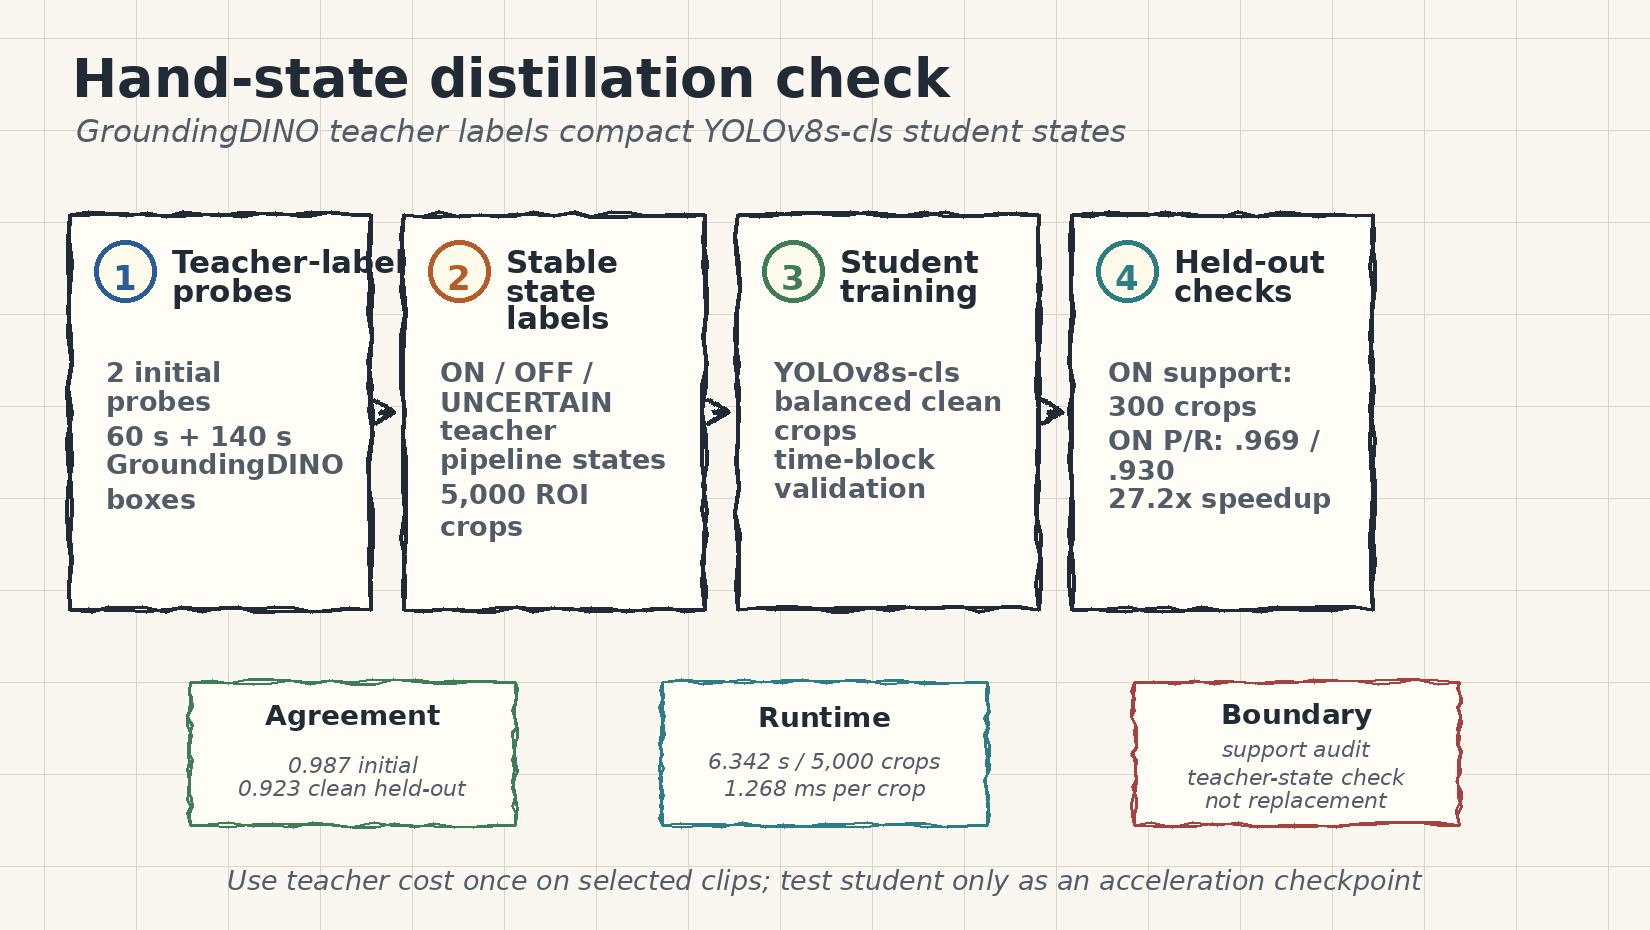
\includegraphics[width=\linewidth]{figures/distillation_schematic.png}
    \Description{A hand-drawn style schematic showing a GroundingDINO
    hand/wheel teacher producing stable ON, OFF, and UNCERTAIN labels for
    ROI crops, a compact YOLOv8s-cls student trained on teacher-labeled crops,
    and independent checks for agreement, runtime, and current scope limits.}
    \caption{State-distillation check for the hand-on-wheel branch.
    GroundingDINO is treated as a teacher on selected probes; the compact
    student is evaluated as an acceleration checkpoint rather than as a
    replacement for full multi-participant validation.}
    \label{fig:distillation_schematic}
\end{figure}

Table~\ref{tab:wheel_distill} summarizes the checks. The initial saved
student matched 1,022/1,035 teacher states (0.987 agreement) and
processed 5,000 crops in 6.342 s after warm-up, versus 172.752 s for the
two GroundingDINO probes (27.2$\times$ speedup), but its \textit{ON}
support was only 12 crops. The ON-enriched clean time-block check raised
\textit{ON} support to 300 held-out crops and reached 0.969 precision,
0.930 recall, and 0.949 F1 for that class. The overall clean held-out
agreement was 0.923, with \textit{OFF} requiring additional
boundary-context review. We therefore treat the student as an
acceleration checkpoint and support audit, not as a production replacement
for the teacher branch.

\begin{table}[t]
\centering
\caption{Teacher-student hand-state distillation checks.}
\label{tab:wheel_distill}
\autouitablefont
\begin{tabular}{llrrrr}
\toprule
Check & State & N & P & R & F1 \\
\midrule
Init. & All & 1,035 & \multicolumn{3}{c}{0.987 agree.; 27.2$\times$ speedup} \\
Init. & OFF & 540 & 0.993 & 0.983 & 0.988 \\
Init. & ON & 12 & 0.857 & 1.000 & 0.923 \\
Init. & UNC. & 483 & 0.986 & 0.992 & 0.989 \\
Clean & All & 900 & \multicolumn{3}{c}{0.923 agree.; support audit} \\
Clean & OFF & 300 & 0.894 & 0.897 & 0.895 \\
Clean & ON & 300 & 0.969 & 0.930 & 0.949 \\
Clean & UNC. & 300 & 0.910 & 0.943 & 0.926 \\
\bottomrule
\end{tabular}
\end{table}

\subsection{Deployment Checks}

Deployment checks support engineering feasibility. In the five-seed LOPO
matrix, all 280 trained models exported to ONNX and no top-1 parity
result fell below 0.99. Table~\ref{tab:deployment} reports a compact CPU
benchmark from the holdout protocol, where all 120 exports completed.
YOLOv8n and YOLOv8s are smaller and faster than non-YOLO backbones,
supporting YOLOv8-cls as a convenient but not uniquely accurate
deployment path.

\begin{table}[t]
\centering
\caption{Compact ONNX CPU deployment benchmark from the holdout protocol.}
\label{tab:deployment}
\autouitablefont
\begin{tabular}{lrrrr}
\toprule
Model & MB & B1 p50 ms & B1 img/s & B32 img/s \\
\midrule
YOLOv8n-cls & 5.5 & 4.85 & 202.2 & 1621.2 \\
YOLOv8s-cls & 19.4 & 5.26 & 183.7 & 903.6 \\
ResNet50 & 89.6 & 7.20 & 139.1 & 525.7 \\
DeiT-Tiny & 21.2 & 17.19 & 56.7 & 291.1 \\
EfficientNet-B0 & 15.3 & 18.63 & 53.4 & 288.3 \\
ConvNeXt-Tiny & 106.2 & 18.65 & 51.8 & 114.1 \\
EfficientNet-B3 & 40.8 & 33.69 & 29.4 & 157.5 \\
\bottomrule
\end{tabular}
\end{table}

\section{Discussion}

The central design choice is auditability: ROI selection, AOI semantics,
participant calibration, temporal stability, hand-state review, and
window aggregation remain separate so errors can be localized rather than
hidden inside an aggregate model score. The evidence also clarifies that
deployment convenience is not unique accuracy. YOLOv8-cls is compact and
exportable, but ResNet50 and EfficientNet-B0 remain competitive for AOI
generalization/adaptation; for hand state, a compact student is useful
only as a support audit until broader human-labeled, multi-context
validation is complete.

For downstream studies, the value is citation-level provenance. A later
analysis can cite this workflow as the source of AOI glance and
hand-on-wheel feature construction while keeping its own claims focused
on behavioral questions, not feature-construction mechanics.

\section{Limitations and Open Work}
\label{sec:remaining_work}

Several limitations remain. The workflow depends on participant labels
and is not a zero-label generalization system. High \textit{Other} rates
can reduce valid-AOI denominators and should be reported downstream. ROI
or layout errors can dominate results, so new layouts, videos, or
manifest edits require repeated review. The hand-on-wheel second pass is
single-reviewer evidence and should be expanded into an independently
double-coded validation set. Window aggregation reduces short-term
flicker and makes behavior summaries auditable, but it does not remove
classifier-derived uncertainty in thresholded episode counts such as long
off-path glances. Current distillation evidence is teacher-state
agreement, not full human-labeled multi-participant validation; the
student must be stress-tested before replacing GroundingDINO. Deployment
benchmarks should be repeated on target hardware before strong latency
claims.

\section{Conclusion}

This WIP presents a human-in-the-loop workflow for extracting AOI-level
glance and hand-on-wheel variables from naturalistic in-cabin video.
Across 15 participants, the workflow processed millions of frames while
retaining reviewable checkpoints for ROI validity, AOI generalization,
participant adaptation, temporal stability, hand-state plausibility,
student acceleration, and deployment feasibility. This result is possible
because the pipeline keeps geometry selection, human AOI semantics,
frame-level inference, temporal smoothing, hand-state review, and
window-level aggregation as separate auditable stages rather than merging
them into a single model score. The evidence therefore supports AutoUI as
a transparent feature-construction method for downstream naturalistic
driving studies, not as an eye-tracking replacement, a production
hand-state detector, or a standalone theory of driver behavior.

\bibliographystyle{ACM-Reference-Format}
\bibliography{method_citation_entries}

\end{document}
